%%This is a very basic article template.
%%There is just one section and two subsections.
\documentclass{article}

\usepackage{graphicx} 
\usepackage{subfigure}

\begin{document}

\title{Power Peering \\ A peer to peer network as a Smtp/Pop3 overlay.}

\author{Omar Moling, Anton Dign\"{o}s \\ Free University of Bozen}

\date{}

\maketitle

\noindent
This report is about the Power Peering application, developed for the course
Computer Networks, held by Prof. Gabriele Gianini, 2008/2009.

\section{Introduction}

Power Peering is an application aimed to be a peer to peer network application
on top of the Smtp and pop3 protocol. Its main features are the one of a common
P2P system, as joining the network, querying resources, requesting resources
and offering such. 

Common P2P applications are based on level 4 protocols as
TCP/IP directly, thous they require special ports of the client to be open, to
work. This application instead uses protocols part of the application layer, to
communicate, this protocols are Smtp for sending and Pop3 for receiving
messages. 

Although it seems to be an overhead to use those message (plain/text)
oriented protocols, its usage has a main advantage. The required ports of this
protocols are already open for mail messaging use and mails are even protected
by the privacy law.

The rest of this report is organized as follows \ldots 
% TODO report organization 


\section{Application Overview}

As already introduced the Power Peering application has as a requirement all
needed functionalities of a P2P system. Figure~\ref{fig:usecasedia} shows the
use case diagram of the application, including all needed functionalities for
the user to work in an abstract way.
\begin{figure}[!hbtp]
\centering
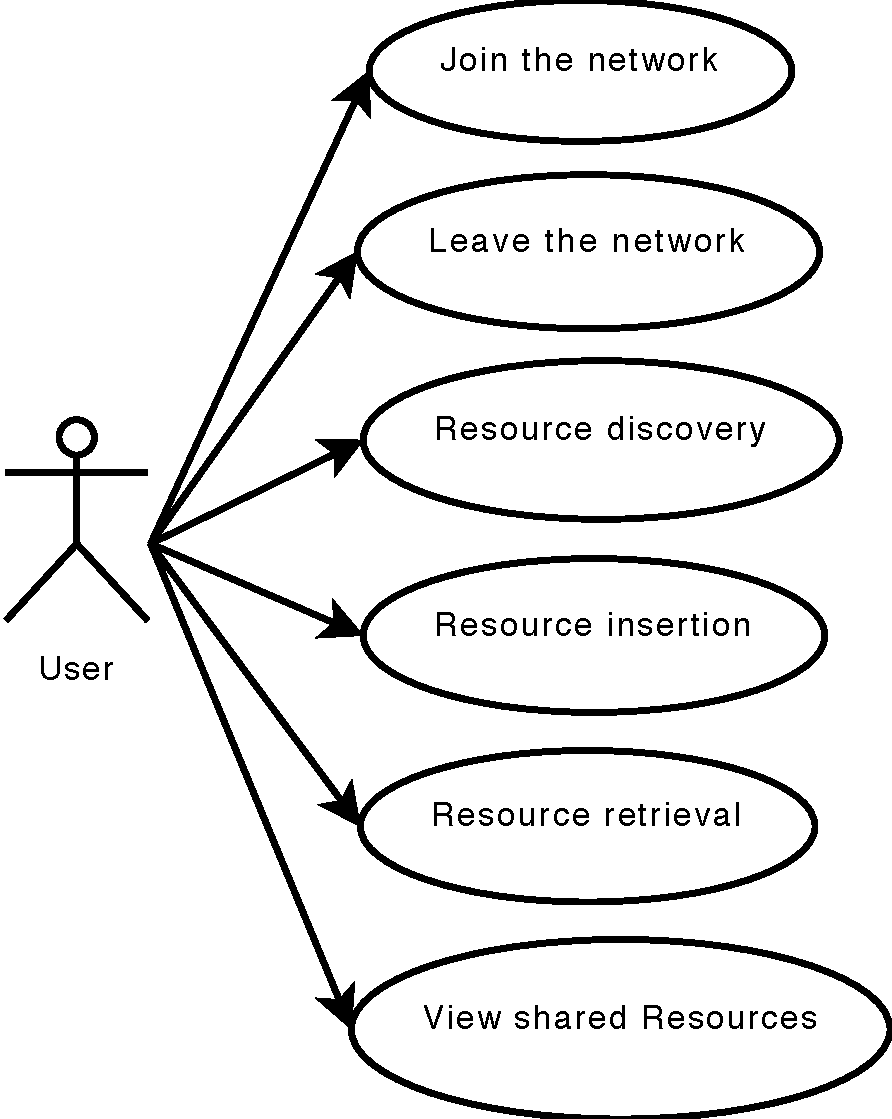
\includegraphics[width=0.4\textwidth]{../img/UseCaseDiagram.pdf}
\caption{Use Case Diagram.}
\label{fig:usecasedia}
\end{figure}
For a better understanding of the systems internal functionality, sequence
diagrams for the most important requirements have been developed.
Figure~\ref{subfig:pingsequence} shows the systems sequence by invoking a
network discovery, which is realized by the internal PING message send to
adjacent clients. These clients forward the the message of the requesting
client and return a PONG message to it. Figure~\ref{subfig:querysequence} shows
instead the sequence of actions performed by the system when a QUERY of a user
is performed. The QUERY is as the PING send to adjacent/intermediate clients,
which forward the message to their adjacent client. The response instead is
always returned directly to the requestor.
\begin{figure}[!hbtp]
\centering
\subfigure[Network joining.]{
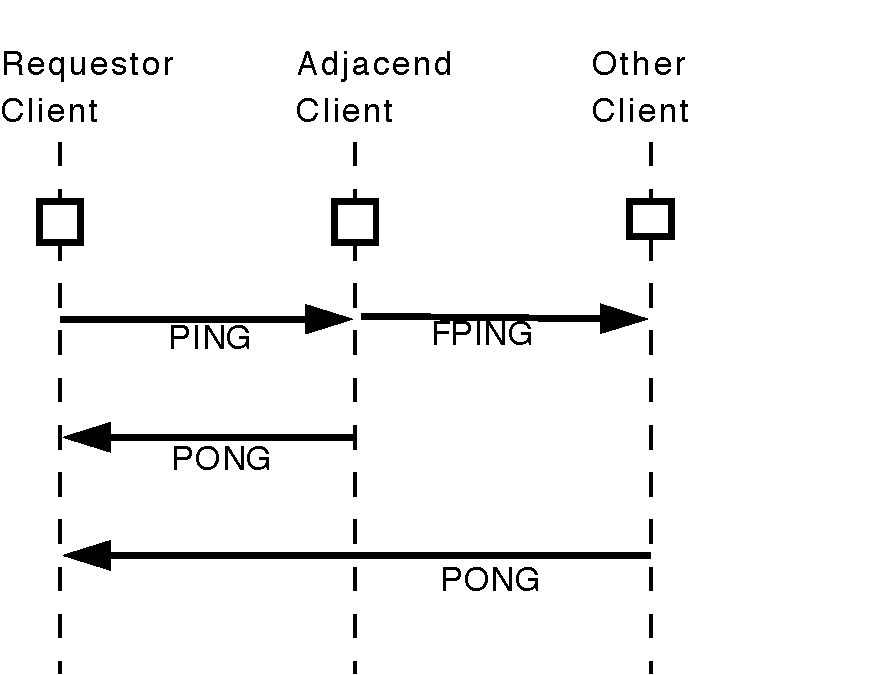
\includegraphics[width=0.4\textwidth]{../img/PingSequenceDiagram.pdf}
\label{subfig:pingsequence}
}
\subfigure[Resource discovery]{
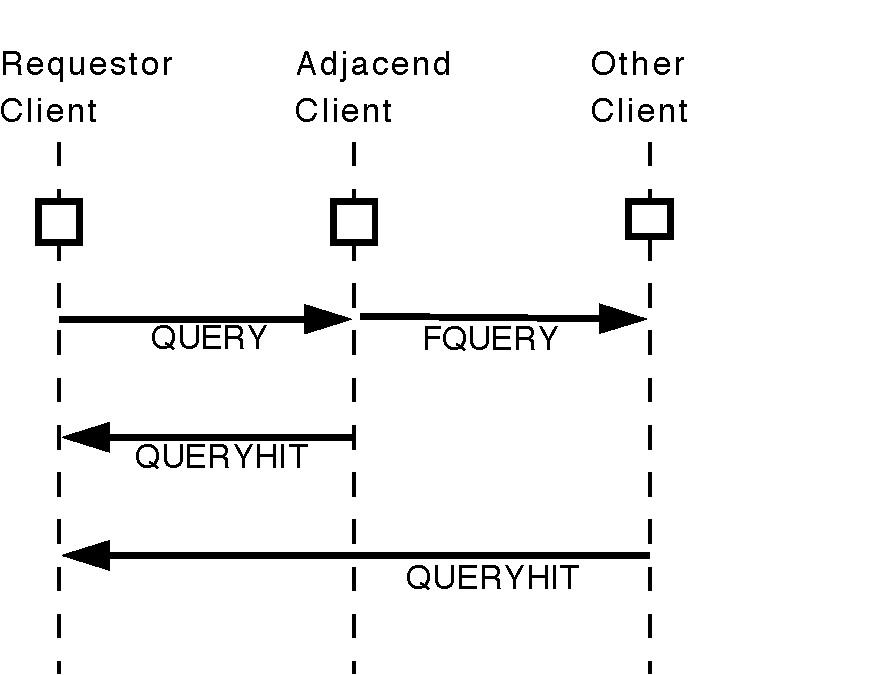
\includegraphics[width=0.4\textwidth]{../img/QuerySequenceDiagram.pdf}
\label{subfig:querysequence}
}
\caption{Sequence Diagrams.}
\label{fig:sequencediagrams}
\end{figure}

The term adjacent client at this point needs an explanation, clients do not
store all other clients of the network and they only keep a subset of them. This
requires a mechanism for forwarding messages as a client can not communicate with
all others. These subset of clients to store is evaluated randomly to avoid
partitioning of the clients, on a PING or PONG request of the network discovery a
client evaluates randomly whether to keep the reference to this client or not
when its client list is already full.

As a client which forwards a message does not know, which of its adjacent
client already got it, messages which need forward contain a field time to
live (TTL) which is decreased by forwarding. A message is not forwarded any
more when its TTL expires.

\section{Application Architecture and Design}

The architecture of the system is divided into 4 packages, reflecting the
components of the application.

\begin{figure}[!hbtp]
\centering
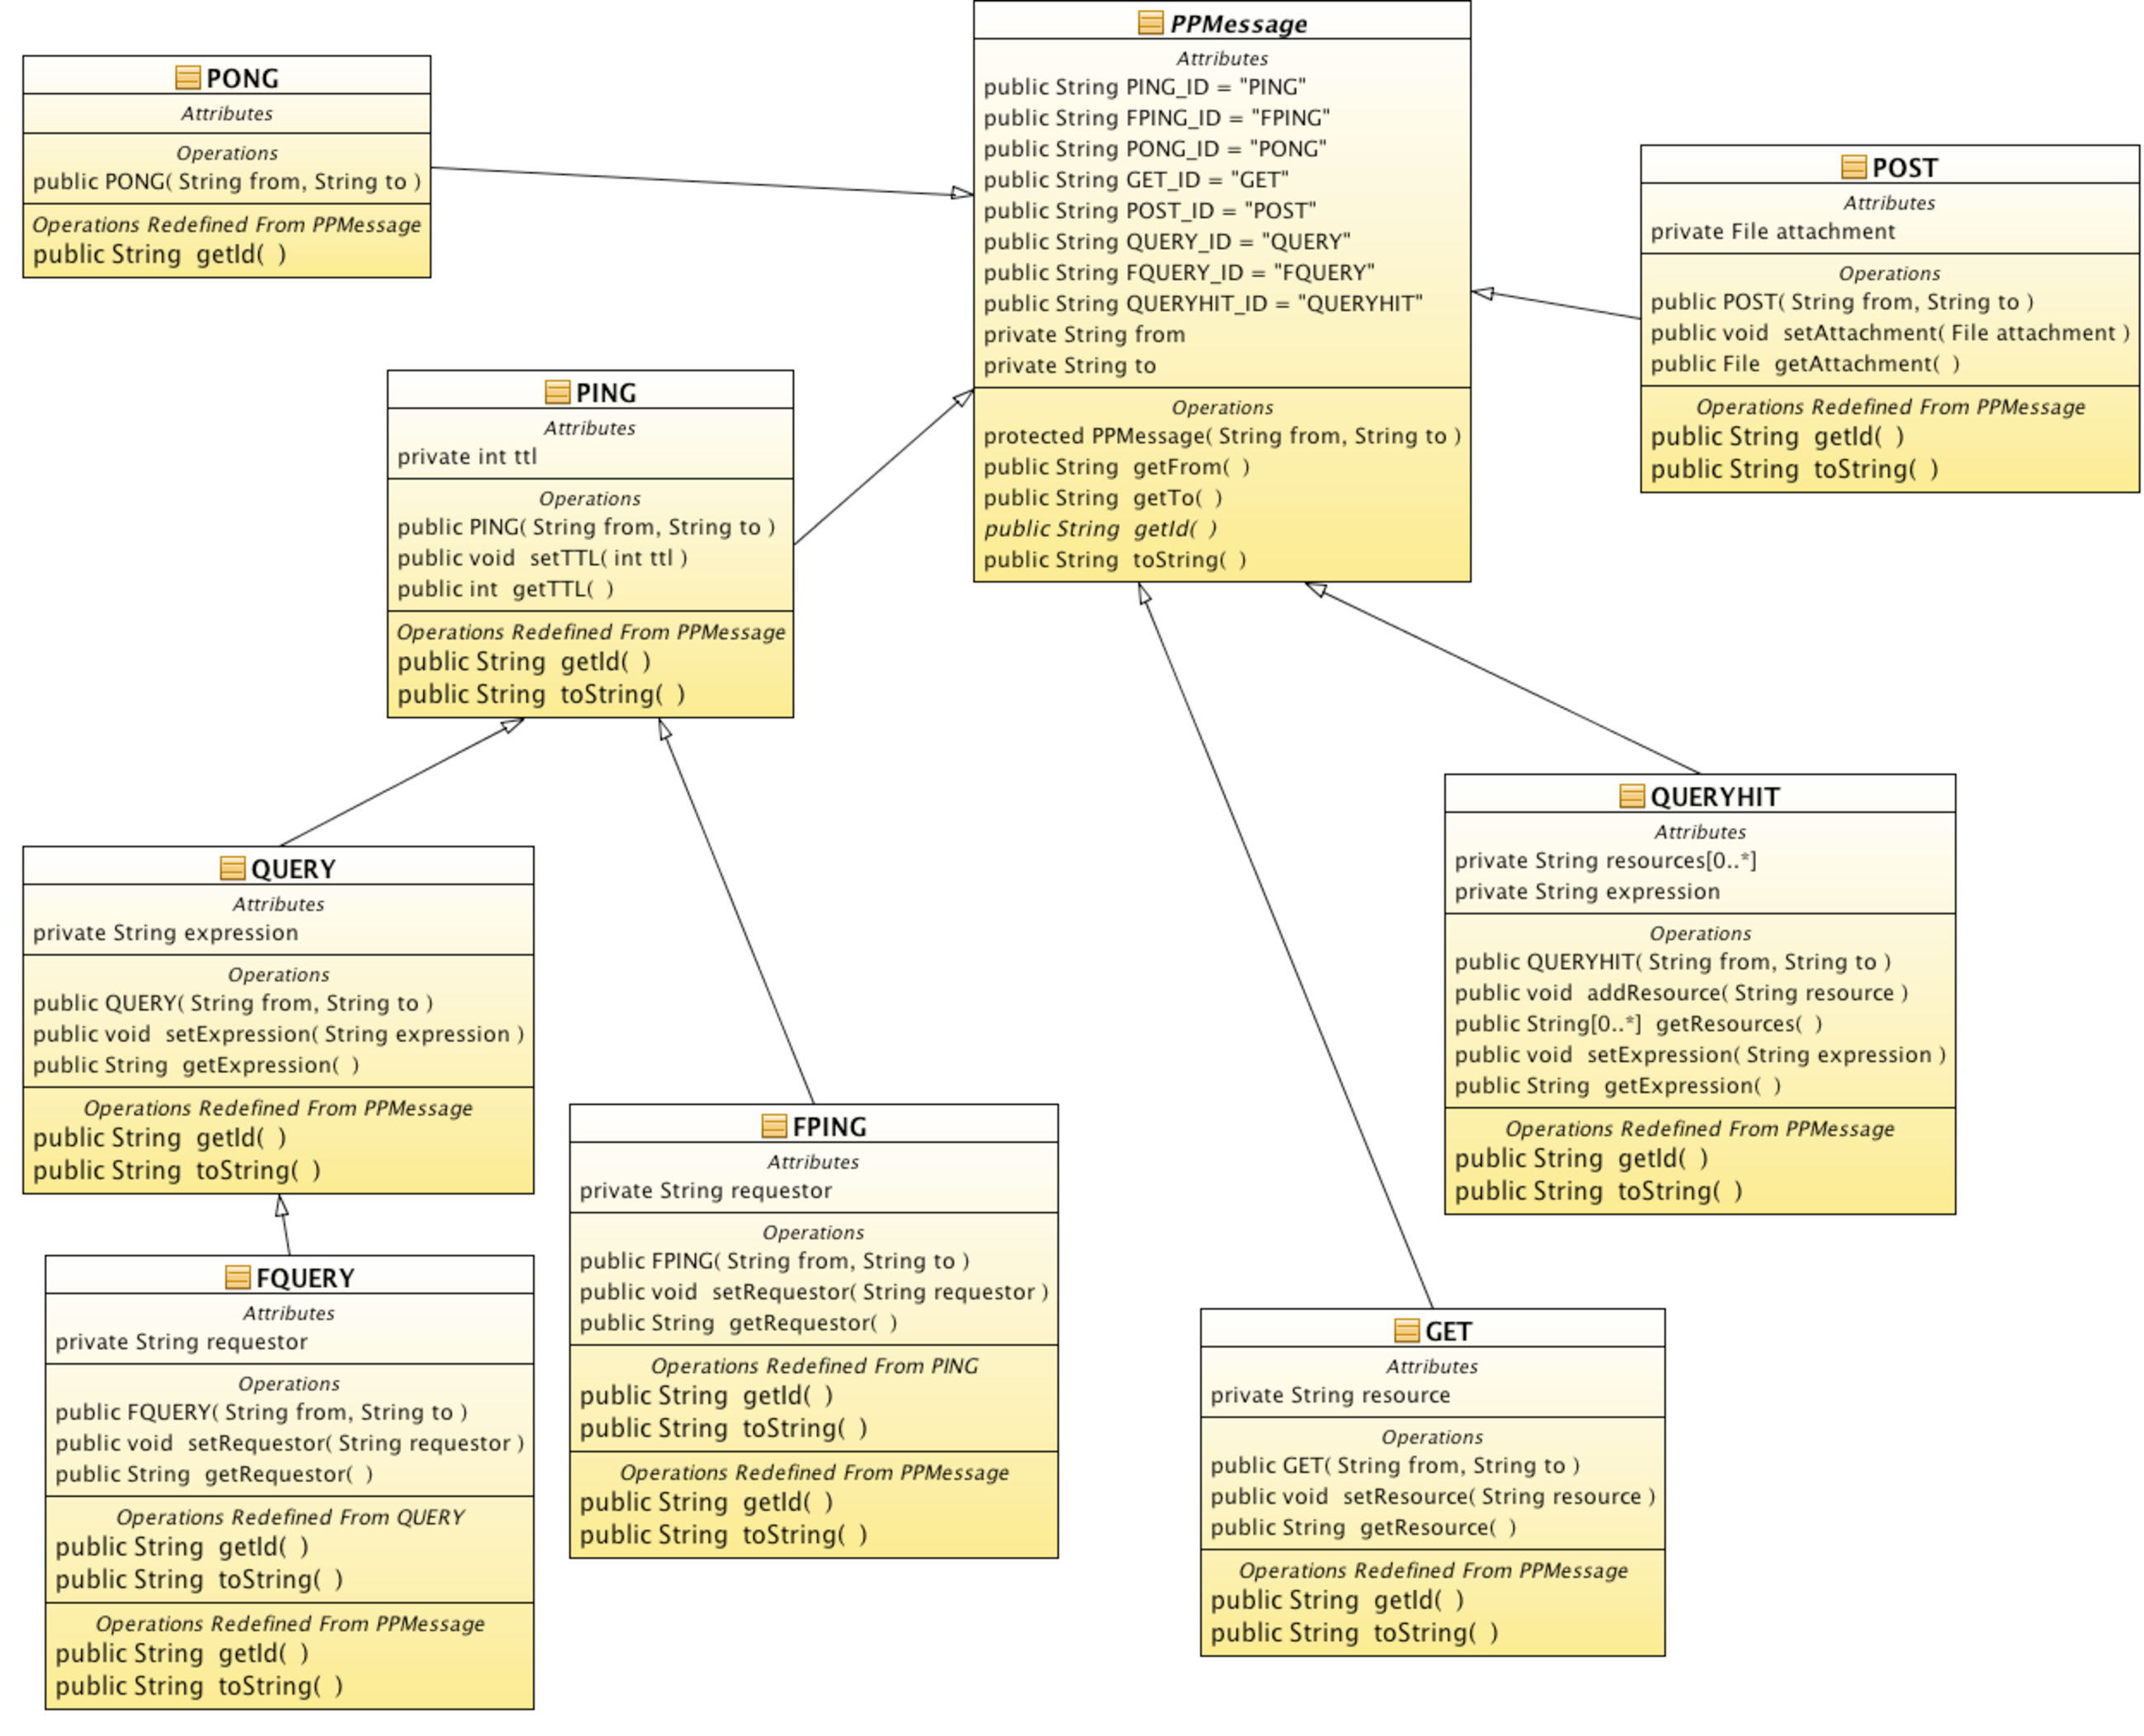
\includegraphics[width=\textwidth]{../img/MessagesClassDiagram.pdf}
\caption{Message Class Diagram.}
\label{fig:messageclassdia}
\end{figure}
Figure~\ref{fig:appclassdia} shows the class diagram of the message package,
these classes are used as data structures for the messages the system ins
capable of sending and/or receiving.

\begin{figure}[!hbtp]
\centering
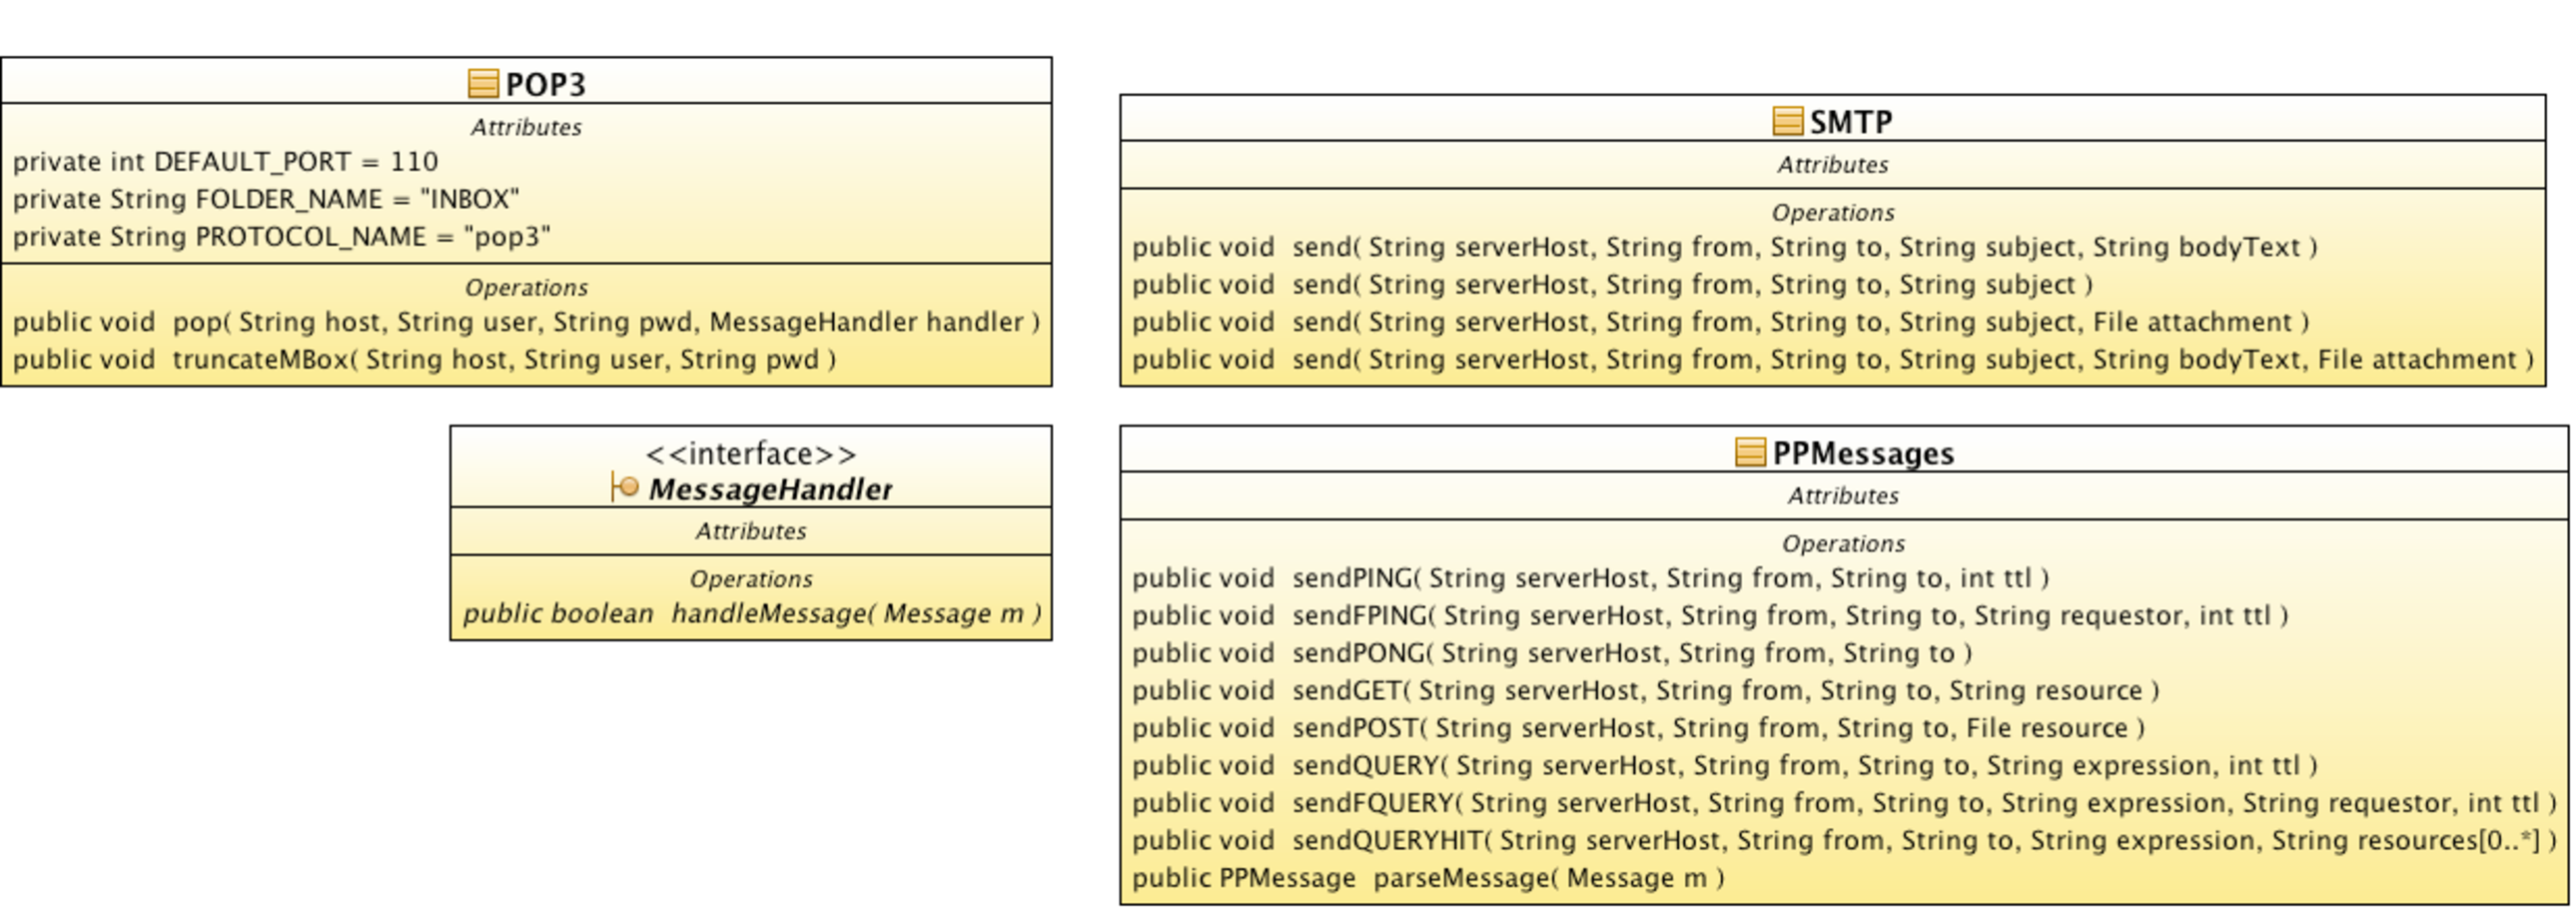
\includegraphics[width=\textwidth]{../img/IoClassDiagram.pdf}
\caption{IO Clas Diagram.}
\label{fig:ioclassdia}
\end{figure}
Figure~\ref{fig:ioclassdia} are the classes of the io package and are responsible
for the abstraction of the protocol overlay. Outside these package classes can
use the PPMessages class to send and parse messages and the POP3 class to fetch
messages, the MessageHandler Interface is used by the POP3 class witch's method
is called for each message of the mail box. These allows the system to only pop
messages which are of its interest, others are left as they are on the server.

\begin{figure}[!hbtp]
\centering
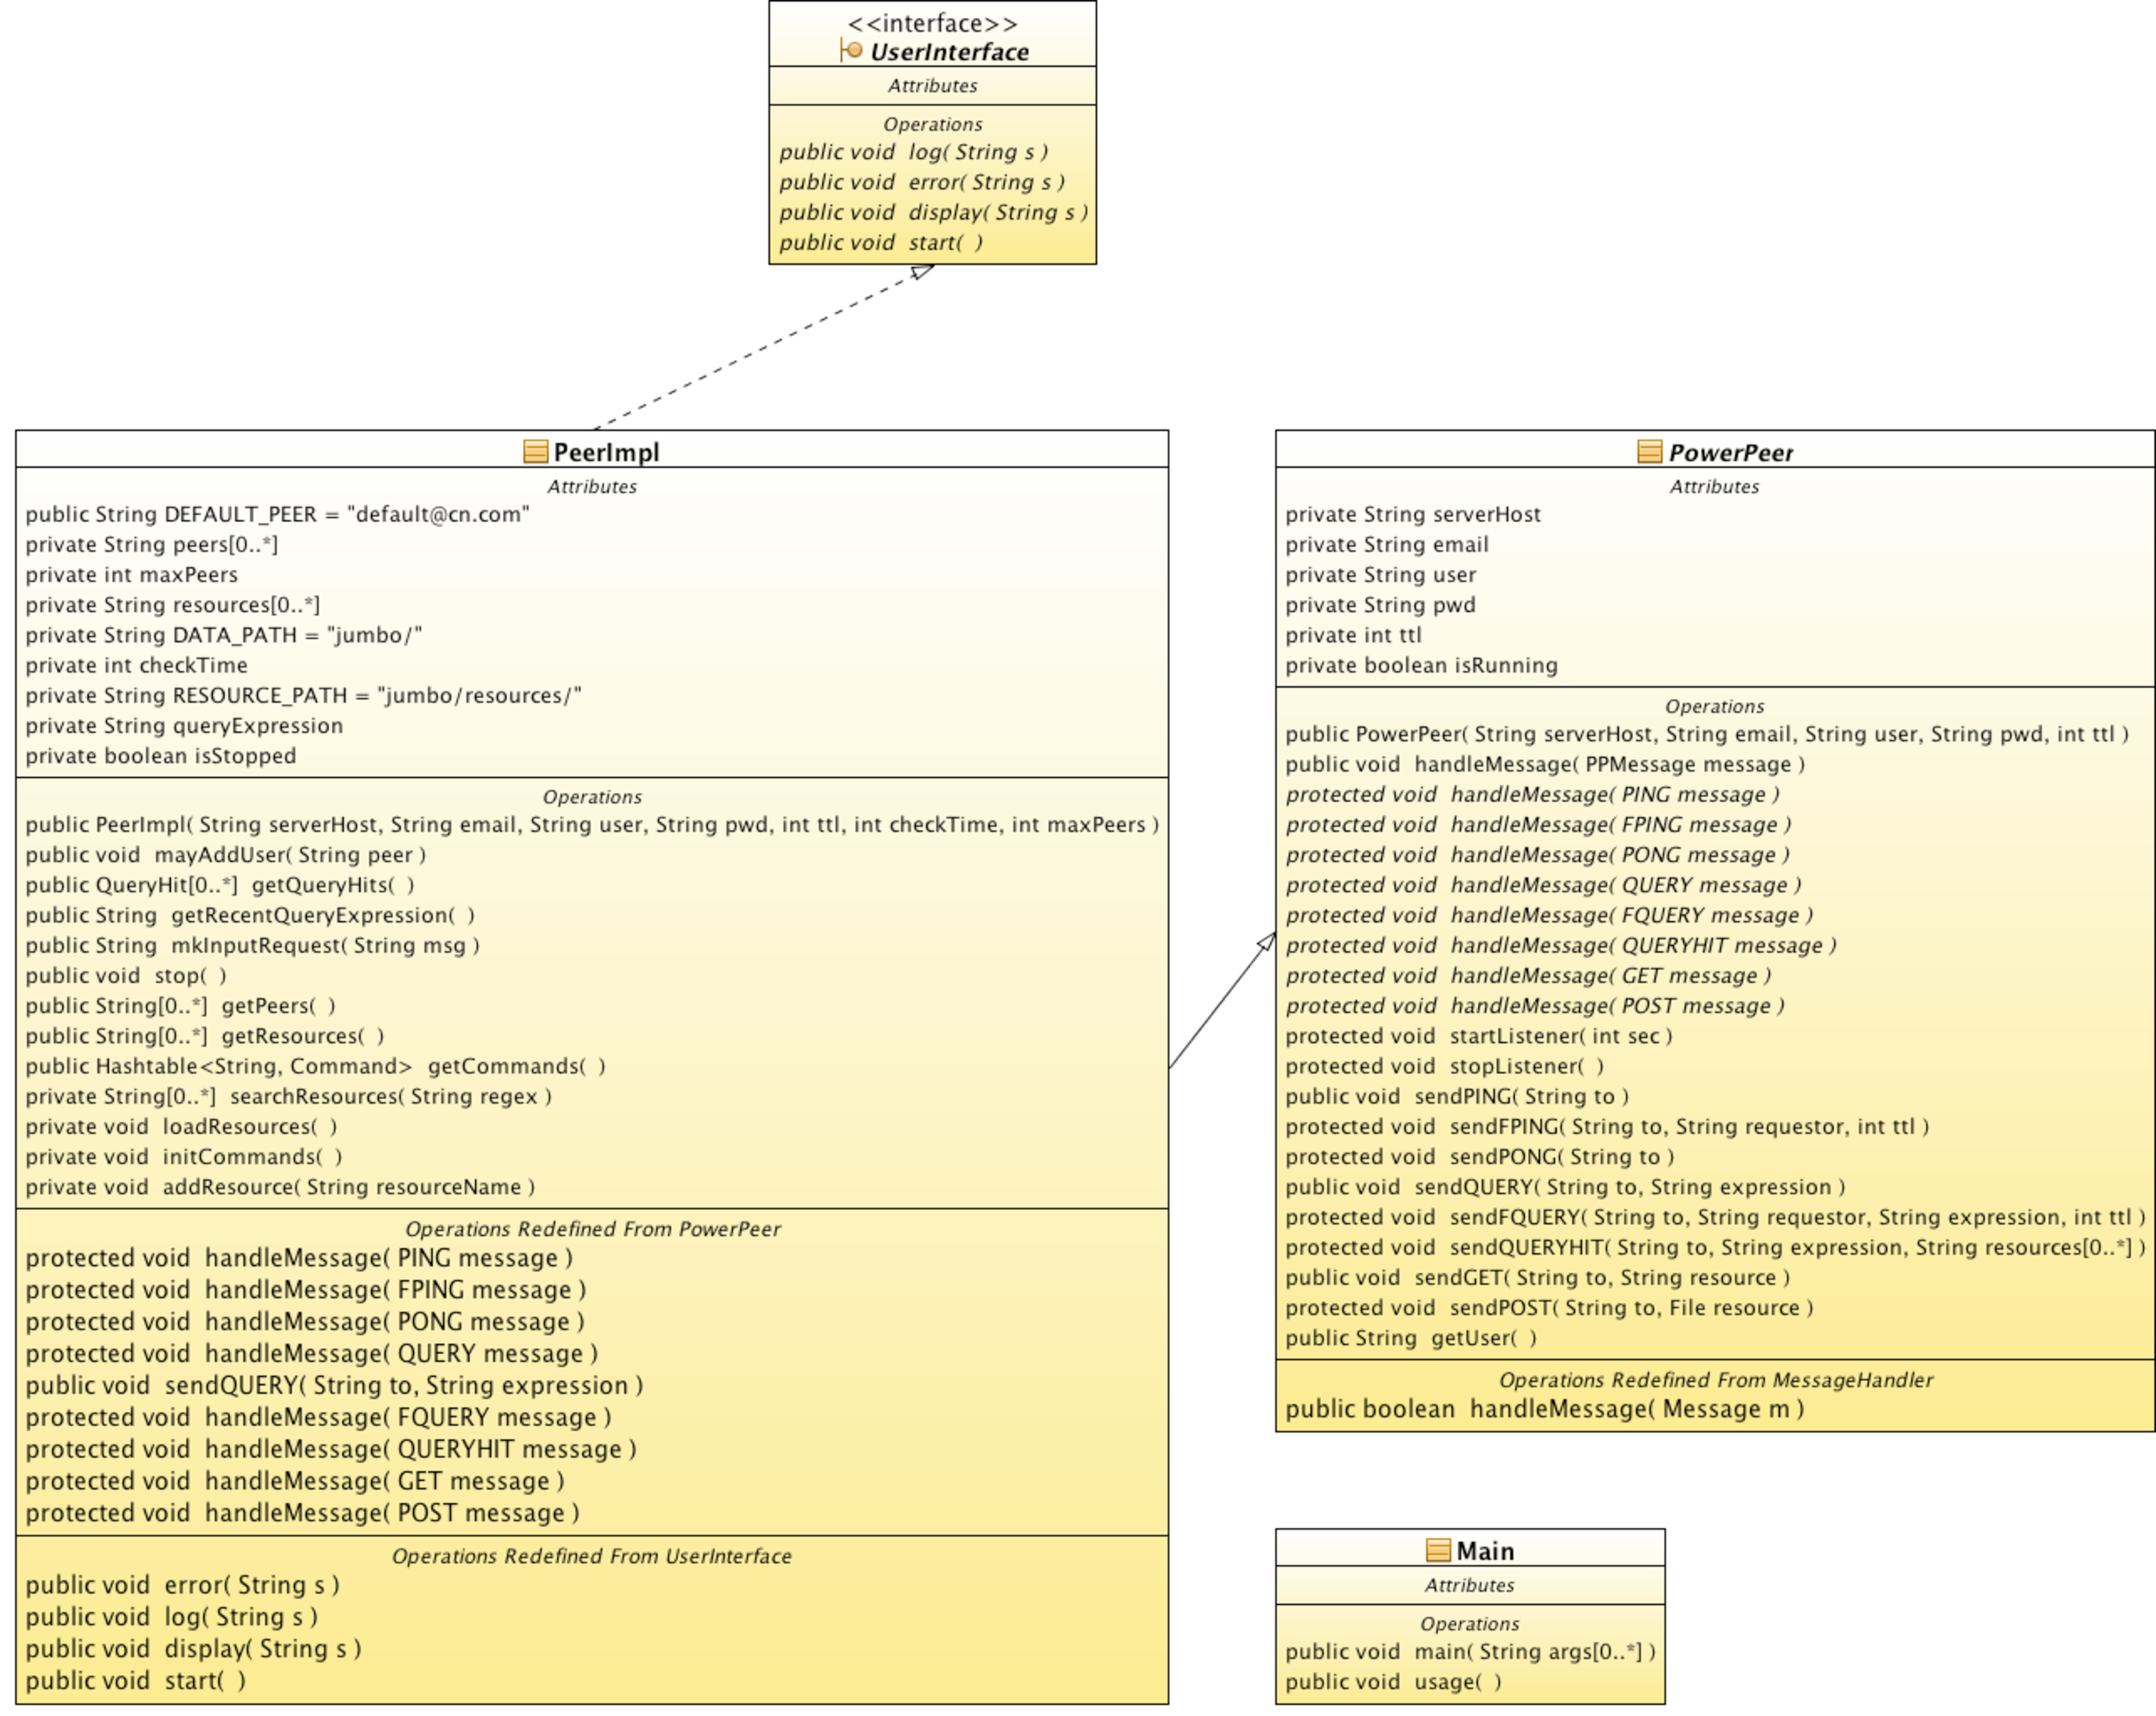
\includegraphics[width=\textwidth]{../img/AppClassDiagram.pdf}
\caption{Application Class Diagram.}
\label{fig:appclassdia}
\end{figure}
Figure~\ref{fig:appclassdia} shows the implementation of the actual client, and
the main entry point of the application. A client can be implemented and
extended by simply extending the PowerPeer class, and extending some of its
methods which are of its interest. The UserInterface interface acts as a common
point for communication with the users output.

\begin{figure}[!hbtp]
\centering
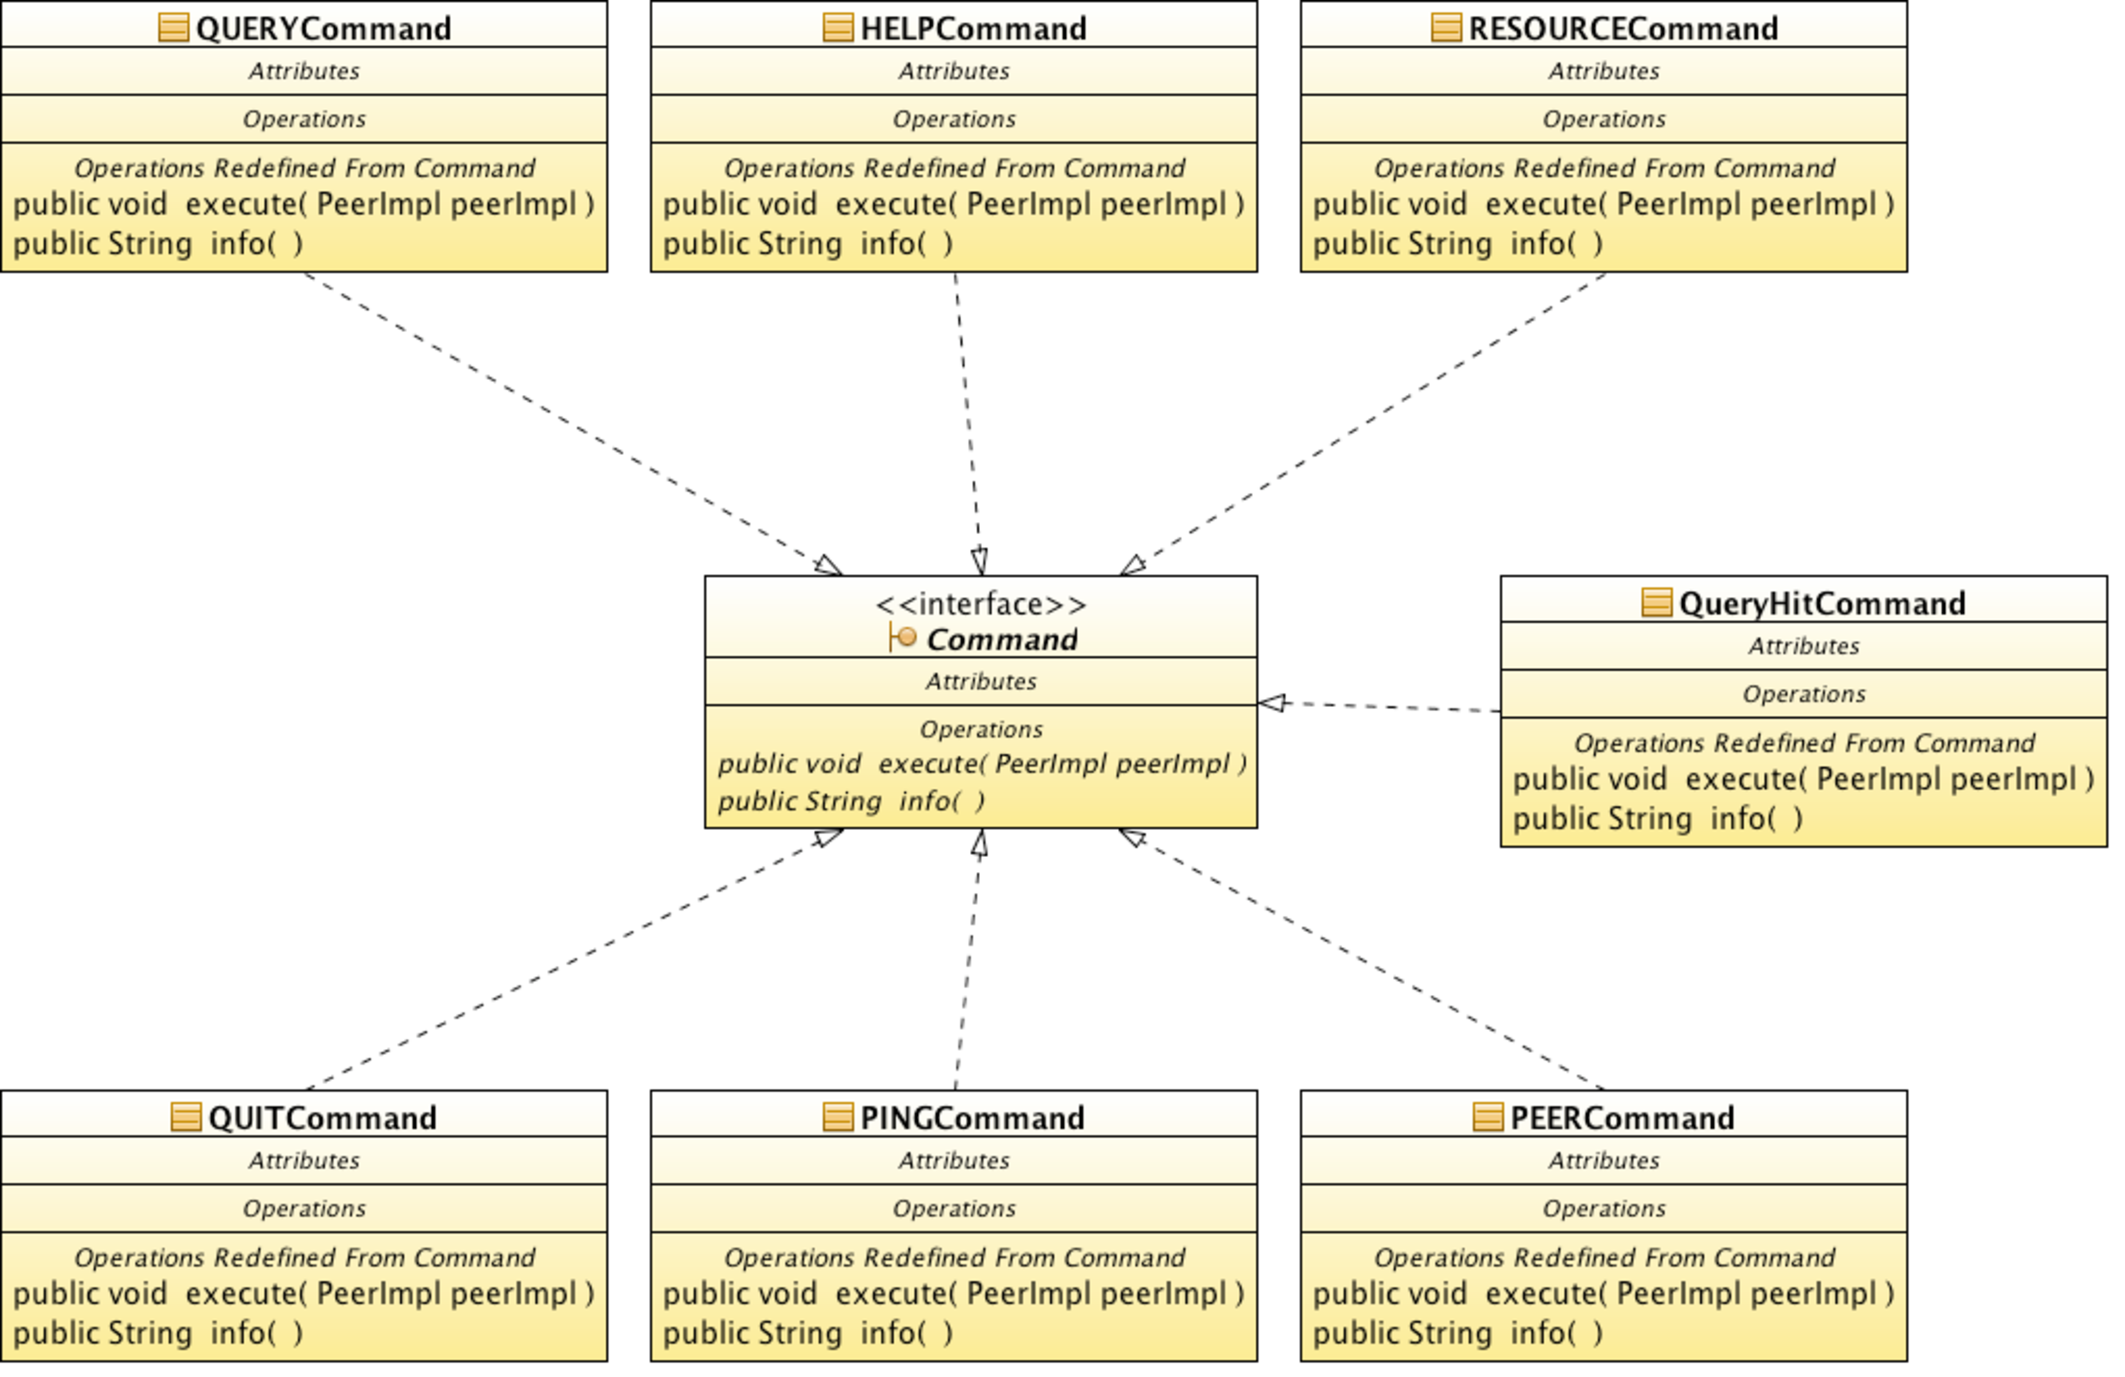
\includegraphics[width=\textwidth]{../img/CommandsClassDiagram.pdf}
\caption{UI Commands Class Diagram.}
\label{fig:commandsclassdia}
\end{figure}
The class diagram shown in Figure~\ref{fig:commandsclassdia} illustrates the
commands used by the Applications user interface. These commands are
implemented and organized by the command design pattern.


\section{Internal Protocol Specification}

This section describes the messages of the system in detail and its
coding/encoding as mail messages.

\subsection{Ping Message}
The ping message acts as the main network join message, which is send to
an initial set of clients aiming to receive an answer who is on the systems
network.
\newline
\noindent
\begin{tabular}{|lll|} 
\hline
field & value & description \\
\hline 
FROM & E-mail address & The requestor client. \\
TO & E-mail address & The destination client. \\
TTL & Integer value & Time to live. \\
\hline 
\end{tabular}

\subsection{FPing Message}
The fping message is the forwarded message of a ping, aiming to enlarge the
message by more adjacency levels.
\newline
\noindent
\begin{tabular}{|lll|} 
\hline
field & value & description \\
\hline 
FROM & E-mail address & The forwarding client. \\
TO & E-mail address & The destination client. \\
TTL & Integer value & Time to live. \\
REQUESTOR & E-mail address & The requestor client. \\
\hline 
\end{tabular}

\subsection{Pong Message}
The pong message is mainly the answer to a PING/FPING messages requestor,
saying that a client is actually in the system.
\newline
\noindent
\begin{tabular}{|lll|} 
\hline
field & value & description \\
\hline 
FROM & E-mail address & The requestor client. \\
TO & E-mail address & The destination client. \\
\hline 
\end{tabular}

\subsection{Query Message}
The query message is the main resource retrieval message, containing a string
as expression for which the requestor is asking for.
\newline
\noindent
\begin{tabular}{|lll|} 
\hline
field & value & description \\
\hline 
FROM & E-mail address & The requestor client. \\
TO & E-mail address & The destination client. \\
TTL & Integer value & Time to live. \\
EXPRESSION & String & The expression of the resource. \\
\hline 
\end{tabular}

\subsection{FQuery Message}
The fquery message is the forwarded message of a query, aiming to enlarge the
message by more adjacency levels.
\newline
\noindent
\begin{tabular}{|lll|} 
\hline
field & value & description \\
\hline 
FROM & E-mail address & The forwarding client. \\
TO & E-mail address & The destination client. \\
TTL & Integer value & Time to live. \\
EXPRESSION & String & The expression of the resource. \\
REQUESTOR & E-mail address & The requestor client. \\
\hline 
\end{tabular}

\subsection{Queryhit Message}
The queryhit message is mainly the answer to a QUERY/FQUERY messages requestor,
saying that a client has a resource matching the query expression.
\newline
\noindent
\begin{tabular}{|lll|} 
\hline
field & value & description \\
\hline 
FROM & E-mail address & The requestor client. \\
TO & E-mail address & The destination client. \\
RESOURCES & String list & The matching resources. \\
\hline 
\end{tabular}

\subsection{Get Message}
The get message is part of the resource retrieval and is the request of a
resource to get.
\newline
\noindent
\begin{tabular}{|lll|} 
\hline
field & value & description \\
\hline 
FROM & E-mail address & The requestor client. \\
TO & E-mail address & The destination client. \\
RESOURCE & String & The requested resource. \\
\hline 
\end{tabular}

\subsection{Post Message}
The post message can be seen as the answere to a get message, containing the
resource of interest of the get's requestor.
\newline
\noindent
\begin{tabular}{|lll|} 
\hline
field & value & description \\
\hline 
FROM & E-mail address & The forwarding client. \\
TO & E-mail address & The destination client. \\
ATTACHMENT & Base64 attachment & The resource of interest. \\
\hline 
\end{tabular}

\subsection{Message Encoding}
As the system uses mail messages to transfer data, all messages have to be
encodes as simple text mail messages. The encoding of these messages has been
realized in a simple manner. The from and to field is used as such in the
email, the subject is used as message specification i.e. which message it
contains and the body is used for all the other content. To identify messages
the header X-Mailer contains PowerPeering as a client.

\section{Application Manual}

\subsection{Installation}

The Power Peering application does not need an installation procedure, the only
required files are the PowerPeering.jar, in the same directory the jumbo
directory has to be present containing the directory resources for shared
resources and an XML-file resources.xml containing the name of the shared
resources.

\subsection{Usage Instructions}

The application can be started by the following command line command:

\noindent
java -jar PowerPeering.jar serverHost email username password

\noindent
This starts the system which allows to perform the following command:
\newline
\noindent
\begin{tabular}{|ll|} 
\hline
command & action performed \\
\hline 
ping &  Send a ping to all adjacent clients. \\
query &  Send a query to all adjacent clients. \\
hits &  See a queryhits returned by the last query. \\
peers & See a list of all adjacent clients. \\
resources &  See a list of all shared resources. \\
help &  See the help of all commands. \\
quit &  Quit the application and all its background threads. \\
\hline 
\end{tabular}


\end{document}
